\documentclass[tikz]{standalone}
\usetikzlibrary{calc}

  \usepackage[no-math]{fontspec}
  \setmainfont{TeXGyreTermes-Regular}[
       BoldFont       = TeXGyreTermes-Bold ,
       ItalicFont     = TeXGyreTermes-Italic ,
       BoldItalicFont = TeXGyreTermes-BoldItalic,
       NFSSFamily     = ntxtlf]
  \setsansfont{TeX Gyre Heros Regular}[
       Scale=.9,
       BoldFont       = TeX Gyre Heros Bold,
       ItalicFont     = TeX Gyre Heros Italic,
       BoldItalicFont = TeX Gyre Heros BoldItalic]
  \setmonofont[StylisticSet={1,3},Scale=.9]{inconsolata}
  \usepackage{newtxmath}
\begin{document}

\definecolor{Maroon}{cmyk}{0, 0.87, 0.68, 0.32}

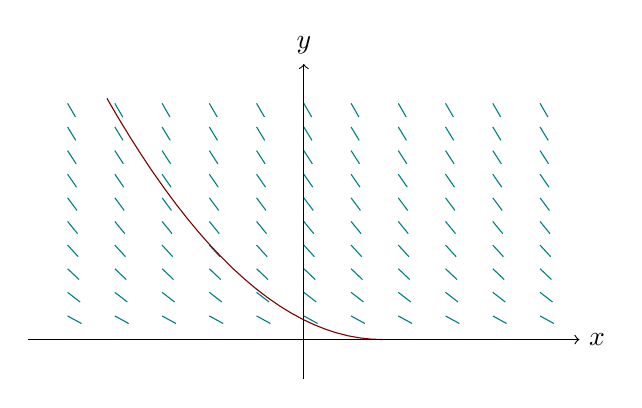
\begin{tikzpicture}[declare function={f(\x,\y)=-\y^(1/2);}]
\def\xmax{3} \def\xmin{-3}
\def\ymax{3} \def\ymin{0}
\def\nx{10}
\def\ny{10}

\pgfmathsetmacro{\hx}{(\xmax-\xmin)/\nx}
\pgfmathsetmacro{\hy}{(\ymax-\ymin)/\ny}
\foreach \i in {0,...,\nx}
\foreach \j in {0,...,\ny}{
\pgfmathsetmacro{\yprime}{f({\xmin+\i*\hx},{\ymin+\j*\hy})}
\draw[teal, shift = {({\xmin+\i*\hx},{\ymin+\j*\hy})}] 
(0,0)--($(0,0)!2mm!(.1,.1*\yprime)$);
}

% Plot a particular solution passing through y0
\draw[color=Maroon] plot[domain=-2.5:1] (\x,{(\x * \x - 2*\x + 1) / 4});

\draw[->] (\xmin-.5,0)--(\xmax+.5,0) node[right] {$x$};
\draw[->] (0,\ymin-.5)--(0,\ymax+.5) node[above] {$y$};
\end{tikzpicture}
\end{document}